

\section*{Solving}

We have system of PDE

\begin{equation}
    \left\{
    \begin{matrix}
    &\frac{\partial^2 u}{\partial x^2} + \frac{\partial^2 u}{\partial y^2} = 0, & in \,  \Omega \, \\
    &u|_{\partial\Omega} = \psi, & on \, \partial \Omega 
    \end{matrix}
    \right.
\end{equation}

And $\psi$ is :

\begin{equation}
\left\{
\begin{matrix}
    &\psi(x,0) = 0, & \psi(x,b) = \sin(x)/\sin(a) & x\, from\, [0,a] \\
    &\psi(0,y) = 0 , & \psi(a,y) = \sinh(y) / \sinh(b) & y\, from \, [0,b]
    \end{matrix}
    \right.
\end{equation}

And if used explicit method

\begin{equation}
    u_{i, j} = \frac{1}{4} (u_{i+1,j} + u_{i-1,j} + u_{i,j+1} + u_{i,j-1}) 
\end{equation}

\begin{figure}[h!]
\centering{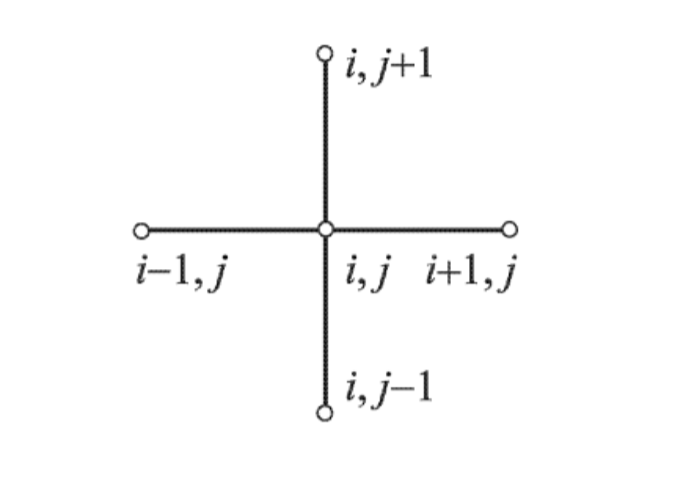
\includegraphics[scale=0.4]{1_1_numerical.png}}
\end{figure}


